\section{Predicción conforme}

%
La Predicción conforme (o inferencia conforme) es un paradigma que utiliza la experiencia pasada para determinar niveles precisos de confianza en las predicciones futuras.
Este no produce una predicción puntual $\hat{y}$ sino que produce una \textbf{región de predicción} $\mathcal{C}(x)$ (un conjunto o un intervalo) estadísticamente rigurosos.
De manera crucial, estos conjuntos son válidos en un sentido libre de distribución: poseen garantías explícitas y no asintóticas incluso sin asumir una distribución de los datos ni supuestos sobre el modelo.


Dada una muestra de prueba $X_{\text{test}}$, se dispone de un modelo previamente entrenado $\hat{f}(\cdot)$ que produce una estimación puntual $\hat{y} = \hat{f}(X_{\text{test}})$. El marco de la Predicción Conforme trata a este predictor como una "caja negra" (\textit{black-box}) totalmente agnóstica.


La predicción conforme opera como una envoltura (\textit{wrapper}) \textbf{post-hoc} sobre cualquier algortimo $\hat{f}$ y proporciona una \text{cobertura marginal}, asegurando que la probabilidad de que la etiqueta verdadera esté contenida en la región de predicción sea mayor o igua que $1 - \alpha$, siendo $\alpha$ el nivel de error elegido por el usuario.

\begin{equation}
1-\alpha \le
\mathbb{P}(y_{\text{test}} \in \mathcal{C}(X_{\text{test}})) <  1-\alpha + \frac{1}{n+1}
\end{equation}



El término \textbf{marginal} indica que esta probabilidad se calcula en promedio sobre la aleatoriedad de todo el conjunto de datos de calibración y de la nueva muestra de prueba $(X_{\text{test}}, Y_{\text{test}})$. Esto garantiza una tasa de acierto global del $(1-\alpha)\%$ a largo plazo, a diferencia de una cobertura condicional puntual $\mathbb{P}(y_{\text{test}} \in \mathcal{C}(X_{\text{test}}) \mid X_{\text{test}} = x)$, la cual requeriría sostener dicha garantía independientemente para cada valor específico de $x$.

Para calibrar el modelo y obtener esta garantía, se agrega una etapa adicional al pipeline tradicional de entrenamiento y evaluación: el paso de calibración. Este consiste en una serie de etapas donde el único supuesto requerido es la \text{intercambiabilidad} de las observaciones $(X_i, Y_i)_{i=1,\dots,n+1}$ (Ver Anexo~\ref{anexo:teorema1}).








Para poder calibrar se debe agregar un paso mas al tipico pipeline de entrenamiento y testeo, se agrega el paso de calibración.

Este consiste en una serie de pasos en donde hay en principio un unico supuesto que se debe cumplir  (Ver Anexo~\ref{anexo:teorema1}) y es el de intercambiabilidad del set de datos $(X_i, Y_i)_{i=1,2,\dots , n}$ donde $(X_i, Y_i) \in \mathcal{X} \times \mathcal{Y}$.


\begin{algorithm}[H]
\caption{Proceso de Calibración en \textit{Conformal Prediction - Framework}}
\label{alg:conformal_prediction}
\begin{algorithmic}[1] % El [1] numera cada paso automáticamente
    \STATE \textbf{Identificar} la noción de heurística o incertidumbre del modelo previamente entrenado.

    \STATE \textbf{Definir} la función de puntuación $s(x,y) \in \mathbb{R}$, también llamada función de no conformidad (los puntajes más grandes definen un peor ajuste entre $x$ e $y$):
    \begin{itemize}
        \item $s(x,y)$ pequeño $\rightarrow$ buen ajuste.
        \item $s(x,y)$ grande $\rightarrow$ mal ajuste.
    \end{itemize}

    \STATE \textbf{Computar} $\hat{q}$ como el percentil de calibración correspondiente al orden $\lceil(n+1)(1-\alpha)\rceil$:
    \begin{equation*}
        \hat{q} = \text{quantile}\left(s_1, \dots, s_n; \frac{\lceil(n+1)(1-\alpha)\rceil}{n}\right)
    \end{equation*}
    donde $s_i = s(X_i, Y_i)$ para $i=1, \dots, n$.

    Esto fija el tamaño del conjunto de predicción de forma que garantiza una cobertura de $1-\alpha$.

    \STATE \textbf{Construir} la región o conjunto de predicción para un nuevo ejemplo $X_{\text{test}}$ utilizando el umbral $\hat{q}$:
    \begin{equation*}
        C(X_{\text{test}}) = \{ y : s(X_{\text{test}}, y) \le \hat{q} \}
    \end{equation*}
    Es decir, el conjunto incluye todos los valores de $y$ que no son ``demasiado improbables'' según el umbral calibrado.
\end{algorithmic}
\end{algorithm}

El Algoritmo \ref{alg:conformal_prediction} define el \textit{framework} general sobre el cual se construyen las distintas técnicas de \textit{Conformal Prediction}.

Este flujo establece una plantilla estándar de calibración: cualquier variante metodológica posterior se reduce, esencialmente, a proponer una definición particular para la función de puntuación de no conformidad $s(x,y)$ en el paso 2, manteniendo el resto del proceso de cuantificación de incertidumbre inalterado con distintas formas de calcular el percentil.

\begin{figure}[H]
    \centering
    \resizebox{1.04\textwidth}{!}{% <-- Cambia 0.95 para agrandar (ej. 1.0) o achicar
        %-------------------------------------------------------------------------%
% ARCHIVO: img_tex/diagrama.tex
% Arreglado con desactivación local para babel (spanish)
%-------------------------------------------------------------------------%
\shorthandoff{>} % Apaga el conflicto del español justo antes de empezar

\begin{tikzpicture}[
    scale=0.85, every node/.style={transform shape},
    % Estilos de los bloques centrales
    bloque/.style={rectangle, draw=gray!60, fill=blue!5, rounded corners=6pt, minimum width=3.5cm, minimum height=1.2cm, align=center, font=\small},
    % Estilo para el texto de las ecuaciones
    textoEq/.style={align=left, font=\small}
]

% 1. FONDOS DE COLORES (Izquierda Verde, Derecha Rosa)
\fill[green!8] (-9, -5.4) rectangle (0, 5.5); % Subí un poquito el fondo (de 5 a 5.5) para que tape la nueva ecuación
\fill[red!5] (0, -5.4) rectangle (9, 5.5);
\draw[gray!30, dashed] (0, -5) -- (0, 5.5); 

% 2. BLOQUES CENTRALES Y FLECHAS
% Agregamos la ecuación arriba de Data en (0, 4.9)
\node[font=\small] (dataset) at (0, 4.99) {$(X_i, Y_i)_{i=1,2,\dots, n}$};

\node[bloque] (data) at (0, 4) {Datos};
\node[bloque] (sistema) at (0, 1.5) {Sistema};
\node[bloque] (cp) at (0, -1.5) {CP \\ $\mathbb{P}(y_{\text{test}} \in \mathcal{C}(X_{\text{test}})) \ge 1-\alpha$};

\node[textoEq] at (0, -4.9) {$y_{test} \mathcal \in {C}(x_{test}) $};

% Flecha delgada desde la nueva ecuación hacia el bloque Data
\draw[->, gray!80, thin] (dataset) -- (data);

\draw[->, gray!80, thick] (data) -- (sistema);
\draw[->, gray!80, thick] (-1, 0.9) -- node[left, black] {$S_i$} (-1, -0.9);
\draw[->, gray!80, thick] (1, 0.9) -- node[right, black] {$\hat{y}_i$} (1, -0.9);
\draw[->, gray!80, thick] (cp) -- (0, -3.5);

% Parámetro alpha apuntando a CP
\draw[->, gray!80, thick] (-2.7, -1.5) node[left, black, font=\large] {$\alpha$} -- (cp);

% 3. LADO IZQUIERDO (Clasificación - Verde)
\node[textoEq] at (-6.5, 1.5) {
    $x_1 \rightarrow \{\hat{y}_2\}$ \\
    $x_2 \rightarrow \{\hat{y}_K\}$ \\
    $\vdots$ \\
    $x_N \rightarrow \{\hat{y}_1\}$
};

\node[textoEq] at (-6.5, -2) {
    $x_1 \rightarrow \{\hat{y}_2, \hat{y}_4, \hat{y}_6\}$ \\
    $x_2 \rightarrow \{\hat{y}_K, \hat{y}_5, \hat{y}_7, \hat{y}_8\}$ \\
    $\vdots$ \\
    $x_N \rightarrow \{\hat{y}_1\}$
};

\node[textoEq] at (-3, -4.2) {$\mathcal{C}(x_{i}) = \{\hat{y}_j, \hat{y}_n, \textcolor{green!60!black}{\hat{y}_{i}}, \hat{y}_k\}$};


% 4. LADO DERECHO (Regresión - Rosa)

% Gráfico Superior (Predicción puntual)
\begin{scope}[shift={(3.5, 0.5)}]
    \draw[->, thick] (0,0) -- (3,0);
    \draw[->, thick] (0,0) -- (0,2);
    % Curva azul de predicción
    \draw[blue!70!cyan, ultra thick] (0.2, 0.4) .. controls (1, 1.5) and (2, 1) .. (2.8, 1.8) node[right, black] {$\hat{y}$};
\end{scope}

% Gráfico Inferior (Intervalos de confianza / bandas)
\begin{scope}[shift={(3.5, -3.2)}]
    \draw[->, thick] (0,0) -- (3,0);
    \draw[->, thick] (0,0) -- (0,2);
    
    % Banda superior (azul claro)
    \draw[blue!30, thick] (0.2, 0.9) .. controls (1, 2) and (2, 1.5) .. (2.8, 2.3);
    % Banda inferior (azul claro)
    \draw[blue!30, thick] (0.2, 0.1) .. controls (1, 1.2) and (2, 0.7) .. (2.8, 1.3);
    % Curva central (gris gruesa)
    \draw[gray!50, line width=3pt] (0.2, 0.5) .. controls (1, 1.6) and (2, 1.1) .. (2.8, 1.8) node[right, black] {$\hat{y}$};
    
    % Etiquetas de las bandas I+ e I-
    \draw[red!70, thick] (2.4, 1.55) -- node[right, font=\tiny] {$I^+$} (2.4, 2.0);
    \draw[red!70, thick] (0.6, 0.5) -- node[right, font=\tiny] {$I^-$} (0.6, 0.85);
\end{scope}

\node[textoEq] at (3.5, -4.2) {$\mathcal{C}(x) = [\hat{y}(x) - I(x), \hat{y}(x) + I(x)]$};

\end{tikzpicture}

\shorthandon{>} % Lo vuelve a encender para que el resto del texto de tu informe funcione bien
    }
    \caption{Esquema general de Conformal Prediction para clasificación y regresión.}
    \label{fig:conformal_prediction}
\end{figure}

El proceso de calibración en el \ref{alg:conformal_prediction} parte del supuesto de intercambiabilidad del conjunto de datos, que es un supuesto mas general que el de iid.

Luego con los datos se debe generar los scores de no conformidad, producto de evaluar los datos en el modelo $\hat{f}$ y extraer del mismo predicciones o scores (salida de softmax) para asi obtener los  scores de no conformidad mediante la funcion de no confomidad seleccionada.

Para el caso de clasificación este funcion de no conformidad puede ser $S(x_i,y_i) = \mathbf{P}(y_i=0  | x_i) = 1 - \mathbf{P}(y_i=1 | x_i)$ (denotado $\hat{\pi}(y|x)$) o para el caso de calibración en regresión puede ser $S(x_i,y_i) = \mid y_i - \hat{y} \mid$ ambas funciones expresan una funcion de no conformidad el cual se las cuales se usaran para decidir que muestras del conjunto de datos de prediccion van a parar dentro del conjunto de prediccion.

\section{Split conformal predictión}

En el algoritmo 1 se mostró el caso general enfocado en clasificación, en la practica se suele hablar de split conformal predictión (SCP), surge a partir del algortimo full conformal prediction que proponia entrenar multiples veces el modelo $\hat{f}$.

En este caso se parte de un set de datos $(X_i, Y_i)_{i=1,2, \dots n}$ el modelo se entrena una vez con los datos $(X_i, Y_i)_{i=1,2, \dots n/2}$ y se calibra con $(X_i,Y_i)_{i=n/2 + 1, \dots , n}$

Se considera el problema de regresión donde $\mathcal{X} \in \mathbb{R}$



\begin{algorithm}[H]
\caption{SCP caso especial - regresión}
\label{alg:conformal_prediction_esp}
    \begin{algorithmic}[1] % Usa [1] para numerar cada línea, o déjalo vacío [] si no quieres números
        \STATE \textbf{Entrenamiento:} Utilizar los datos $(X_i, Y_i)$ para $i = 1, \dots, \frac{n}{2}$ para ajustar un modelo predictivo $\hat{f} : \mathcal{X} \to \mathbb{R}$.

        \STATE \textbf{Cálculo de residuos:} Para $i = \frac{n}{2} + 1, \dots, n$, calcular el residuo absoluto $S_i = |Y_i - \hat{f}(X_i)|$.

        \STATE \textbf{Cálculo del cuantil:} Ordenar los residuos $S_{\frac{n}{2}+1}, \dots, S_n$ en orden creciente, y definir $\hat{q}$ como el elemento de valor $\lceil(1 - \alpha)(\frac{n}{2} + 1)\rceil$ en la lista ordenada.
        Entonces, $\hat{q} = \text{quantile}\left(s_1, \dots, s_n; \frac{\lceil(n+1)(1-\alpha)\rceil}{n}\right)$.

        \STATE \textbf{Inferencia:} Devolver el intervalo de predicción $\mathcal{C}(X_{n+1}) = [\hat{f}(X_{n+1}) - \hat{q}, \hat{f}(X_{n+1}) + \hat{q}]$.
    \end{algorithmic}
\end{algorithm}

El algortimo dos a diferencia del algortimo 1 el conjunto de prediccion devuelto es un intervalo $\mathcal{C}(X_{n+1}) = [\hat{f}(X_{n+1}) - \hat{q}, \hat{f}(X_{n+1}) + \hat{q}]$ el cual representa la incerteza alrededor de la prediccion $\hat{f}(X_{n+1})$ para el target $Y_{n+1}$.

El valor de $\hat{q}$ es una constante que se calcula con los datos de calibración $(X_i,Y_i)_{i=n/2, \dots, n}$ y en esos datos se eleigio $\hat{q}$ de forma que cumpla que los $Y_i$ esten contenidos en el intervalo una fracción de $1-\alpha$

siendo los datos iid luego cualquier nueva prediccion va a cumplir la garantia marginal.


\begin{algorithm}[H]
\caption{SCP caso general}
\label{alg:conformal_prediction_gen}
    \begin{algorithmic}[1]
    \STATE \textbf{Construcción de la función de puntuación:} Utilizar los datos $(X_i, Y_i)$ para $i = 1, \dots, n/2$ para construir una \textbf{score de no conformida} $s : \mathcal{X} \times \mathcal{Y} \to \mathbb{R}$.
    La intuición es que $s(x, y)$ mide qué tan "inusual"  es el punto $(x, y)$ basándose en un modelo ajustado con los datos de esta primera mitad.

    \STATE \textbf{Cálculo de puntuaciones:} Para $i = n/2 + 1, \dots, n$, calcular la puntuación $S_i = s(X_i, Y_i)$ para cada dato en el conjunto de calibración.

    \STATE \textbf{Cálculo del cuantil:} Ordenar las puntuaciones $S_{n/2+1}, \dots, S_n$ en orden creciente, y definir $\hat{q}$ como el elemento de valor $\lceil(1 - \alpha)(\frac{n}{2} + 1)\rceil$ en la lista ordenada.

    \STATE \textbf{Inferencia:} Devolver el conjunto de predicción $\mathcal{C}(X_{n+1}) = \{y \in \mathcal{Y} : s(X_{n+1}, y) \leq \hat{q}\}$.
    \end{algorithmic}
\end{algorithm}

En el algortimo 3 vemos que en realidad SCP no es solo de regresion sino que se ajusta a los dos casos vistos en este problema, y en general todos los otros casos que veremos en siguientes secciones se deberian poder aplicar para ambos problemas de calibración.


\section{Scores de no conformidad}

Los \textbf{scores de no conformidad} son el concepto fundamental del marco de predicción conforme.

Se definen como una función $s(x, y)$ diseñada de tal manera que \textbf{valores más altos indican que el punto de datos $(x, y)$ no concuerda con las tendencias observadas} en los datos de entrenamiento.

\begin{itemize}
    \item Propósito: Actúa como una métrica que mide qué tan grande es el error del modelo en un dato nuevo frente a los datos con los que fue entrenado.

    \item Flexibilidad y Garantía: Puedes elegir prácticamente cualquier función de puntuación; siempre que sea simétrica, el método garantiza matemáticamente el nivel de confianza objetivo (por ejemplo, 95\% de cobertura), sin importar si el modelo es excelente o deficiente.

    \item Impacto Práctico: La elección del score es lo mas importante. Aunque la validez estadística no cambia, un buen score optimiza el método generando intervalos de predicción pequeños, precisos y realmente útiles (eficientes).
\end{itemize}


\textbf{Tipos comunes de funciones de puntuación}

\begin{itemize}
    \item \textbf{Score de residuo absoluto:} Definido como $s(x, y) = |y - \hat{f}(x)|$. Produce bandas de confianza de \textbf{ancho constante} alrededor de la predicción puntual.

    \item \textbf{Score de residuo escalado:} Se define como $s(x, y) = \frac{|y - \hat{f}(x)|}{ \hat{\sigma}(x)}$.
    Permite que el ancho del intervalo se adapte según una estimación de la varianza del ruido $\hat{\sigma}$, siendo más útil cuando el ruido no es constante.


    EL resultado de la predecicción será:

    $$
    \mathcal{C}(X_{n+1}) = \hat{f}(X_{n+1}) \pm \hat{q} . \hat{\sigma} (X_{n+1})
    $$

    \item \textbf{Score CQR (Conformalized Quantile Regression):}
    Utiliza estimaciones iniciales de cuantiles para medir la \textbf{distancia con signo} (o distancia algebraica) del valor real $y$ al intervalo condicional estimado $[\hat{\tau}(x; \alpha/2), \hat{\tau}(x; 1 - \alpha/2)]$. Es un enfoque no paramétrico que permite obtener \textbf{intervalos asimétricos y adaptativos} a la distribución local de los datos.

    El score conforme para cada punto se define como:
    $$
    s(x, y) = \max \left\{ \hat{\tau}(x; \alpha/2) - y, \, y - \hat{\tau}(x; 1 - \alpha/2) \right\}
    $$
    Un valor positivo de $s(x,y)$ indica que el dato real quedó fuera del intervalo de los cuantiles estimados, mientras que un valor negativo indica que cayó dentro.

    A partir de la calibración de este score, el conjunto de predicción final para un nuevo punto de prueba $X_{n+1}$ se ajustando el intervalo inicial mediante el cuantil empírico corregido $\hat{q}$:
    $$C(X_{n+1}) = \left[ \hat{\tau}(X_{n+1}; \alpha/2) - \hat{q}, \, \hat{\tau}(X_{n+1}; 1 - \alpha/2) + \hat{q} \right]$$

    \item \textbf{Score de Alta Probabilidad (High-Probability Score):}
    Se utiliza en problemas de clasificación donde la variable de respuesta toma valores en un conjunto discreto de etiquetas $\{1, \dots, K\}$. A partir de un modelo que estima la probabilidad condicional $\hat{\pi}(y \mid x)$, el score de inconformidad se define como el negativo de dicha probabilidad:
    $$s(x, y) = -\hat{\pi}(y \mid x)$$
    El signo negativo asegura la propiedad fundamental de Conformal Prediction: el score devuelve valores más altos (más cercanos a cero) cuando el punto de datos $(x, y)$ es más improbable.

    Tras calcular el cuantil de calibración $\hat{q}$, el conjunto de predicción final $C(X_{n+1})$ para un nuevo dato de prueba incluye a todas las etiquetas que posean una probabilidad estimada lo suficientemente alta:
    $$C(X_{n+1}) = \{y : \hat{\pi}(y \mid X_{n+1}) \ge -\hat{q}\} \subseteq \{ 1, \dots K \} $$

    La forma general es decir que $t^*(x) = -\hat{q}$ un umbral de decisión.

    %\item \textbf{Score de probabilidad acumulativa:}
    %También llamado score adaptativo, agrupa clases sumando sus probabilidades hasta alcanzar un umbral, lo que ayuda a aproximar la cobertura condicional en clasificación.

\end{itemize}


\begin{figure}[H]
    \centering
    \resizebox{1.0\textwidth}{!}{%-------------------------------------------------------------------------%
% ARCHIVO: img_tex/diagrama_completo.tex
% Versión corregida de ALTA FIDELIDAD - Método Hercule Poirot
%-------------------------------------------------------------------------%
\shorthandoff{>} % Evita conflictos con babel spanish

% 1. DEFINICIÓN DE DATOS GLOBALES
\newcommand{\puntosRegresion}{
    0.4/2.6, 0.4/3.0, 0.5/2.9, 0.5/2.4, 0.6/2.7, 0.7/2.5, 0.7/2.2, 0.8/2.7, 
    0.9/2.4, 1.0/2.2, 1.1/2.0, 1.2/1.5, 1.3/2.3, 1.3/1.9, 1.4/1.6, 1.5/2.1, 
    1.6/1.8, 1.7/1.5, 1.8/1.7, 1.8/2.2, 1.9/1.9, 2.0/1.5, 2.1/1.6, 2.2/2.1, 
    2.3/1.8, 2.3/2.5, 2.4/2.4, 2.4/2.7, 2.5/2.6, 2.5/2.9, 2.6/2.0, 2.7/1.8, 
    2.7/2.2, 2.8/2.4, 2.8/1.6, 2.9/1.3, 2.9/2.4, 3.0/1.4, 3.0/2.1, 3.1/1.6, 
    3.2/1.5, 3.3/1.1, 3.3/2.3, 3.4/1.3, 3.4/1.8, 3.5/0.8, 3.6/0.9, 3.6/1.2, 
    3.7/1.1, 3.8/0.6, 3.9/0.4, 4.0/0.5
}

% Trayectoria de la línea de predicción central
\newcommand{\lineaPrediccion}{
    (0.5, 2.8) .. controls (1.0, 2.0) and (1.5, 1.7) .. (2.3, 1.7)
               .. controls (3.0, 1.7) and (3.5, 1.2) .. (4.0, 0.7)
}

\begin{tikzpicture}[
    scale=0.8, every node/.style={transform shape},
    eje/.style={thick, draw=black!80},
    punto/.style={circle, fill=black!50, inner sep=0.4pt},
    barra_in/.style={draw=black!70, fill=yellow!60, line width=0.5pt},
    barra_out/.style={draw=black!70, fill=gray!40, line width=0.5pt},
    banda/.style={fill=blue!20!cyan!20, opacity=0.6}
]

% =========================================================================
% FILA SUPERIOR: REGRESIÓN
% =========================================================================

% --- GRÁFICO 1: Residual Score (Ancho Constante) ---
\begin{scope}[shift={(0,5)}]
    \node[font=\large\bfseries, text=black!70] at (2.2, 3.8) {Score residual };
    \draw[eje] (0,0) -- (4.5,0) node[below left] {$\mathcal{X}$};
    \draw[eje] (0,0) -- (0,3.5) node[above left] {$\mathcal{Y}$};
    
    \fill[banda] 
        (0.5, 3.3) .. controls (1.0, 2.5) and (1.5, 2.2) .. (2.3, 2.2) 
                   .. controls (3.0, 2.2) and (3.5, 1.7) .. (4.0, 1.2) --
        (4.0, 0.2) .. controls (3.5, 0.7) and (3.0, 1.2) .. (2.3, 1.2)
                   .. controls (1.5, 1.2) and (1.0, 1.5) .. (0.5, 2.3) -- cycle;
                   
    \draw[gray!60, thick] \lineaPrediccion;
    
    % Expansión controlada y limpia mediante una macro temporal ejecutada al instante
    \edef\ejecutarLoopUno{\noexpand\foreach \noexpand\x/\noexpand\y in {\puntosRegresion}{\noexpand\node[punto] at (\noexpand\x,\noexpand\y) {};}}
    \ejecutarLoopUno
\end{scope}

% --- GRÁFICO 2: Scaled Residual Score (Efecto Globo Central) ---
\begin{scope}[shift={(5.5,5)}]
    \node[font=\large\bfseries, text=black!70] at (2.2, 3.8) {Residuo scalado};
    \draw[eje] (0,0) -- (4.5,0) node[below left] {$\mathcal{X}$};
    \draw[eje] (0,0) -- (0,3.5) node[above left] {$\mathcal{Y}$};

    \fill[banda] 
        (0.5, 2.92) .. controls (0.79, 2.58) and (0.92, 2.42) .. (1.25, 2.22)
                    .. controls (2.12, 1.82) and (2, 2.58) .. (2.8, 2.58)
                    .. controls (3.48, 2.32) and (3.01, 1.69) .. (4.03, 1.1) --
        (4.03, 0.4) .. controls (3.5, 0.82) and (3.25, 1.18) .. (2.25, 1.08)
                    .. controls (1.58, 1.25) and (1.52, 1.62) .. (1.12, 1.87)
                    .. controls (0.72, 2.18) and (0.63, 2.28) .. (0.5, 2.38) -- cycle;
                    
    \draw[gray!60, thick] \lineaPrediccion;
    
    \edef\ejecutarLoopDos{\noexpand\foreach \noexpand\x/\noexpand\y in {\puntosRegresion}{\noexpand\node[punto] at (\noexpand\x,\noexpand\y) {};}}
    \ejecutarLoopDos
\end{scope}

% --- GRÁFICO 3: Quantile Regression Score (CQR Asimétrico) ---
\begin{scope}[shift={(11,5)}]
    \node[font=\large\bfseries, text=black!70] at (2.2, 3.8) {Score CQR};
    \draw[eje] (0,0) -- (4.5,0) node[below left] {$\mathcal{X}$};
    \draw[eje] (0,0) -- (0,3.5) node[above left] {$\mathcal{Y}$};
    
    \fill[banda] 
        (0.5, 2.92) .. controls (0.79, 2.58) and (0.92, 2.42) .. (1.25, 2.22)
                    .. controls (2.12, 1.82) and (2, 2.75) .. (2.75, 3)
                    .. controls (3.71, 2.82) and (3.01, 1.69) .. (4.03, 1.1) --
        (4.03, 0.4) .. controls (3.38, 0.67) and (3.31, 1.08) .. (2.88, 1.42)
                    .. controls (2.45, 1.62) and (2.08, 1.48) .. (1.5, 1.62)
                    .. controls (1, 2.13) and (0.68, 2.28) .. (0.5, 2.38) -- cycle;

    \draw[gray!60, thick] \lineaPrediccion;
    
    \edef\ejecutarLoopTres{\noexpand\foreach \noexpand\x/\noexpand\y in {\puntosRegresion}{\noexpand\node[punto] at (\noexpand\x,\noexpand\y) {};}}
    \ejecutarLoopTres
\end{scope}

% =========================================================================
% FILA INFERIOR: CLASIFICACIÓN
% =========================================================================
\begin{scope}[shift={(84pt,-6pt)}]
    \draw[thick] (0,0) -- (9.5,0) node[below left] {$\mathcal{Y}$}; 
    \draw[thick] (0,0) -- (0,3.2); 
    
    \node[font=\LARGE] at (0.8, 3.3) {$\hat{\pi}(y \mid x)$};
    \node[font=\LARGE\bfseries] at (6.46, 3.3) {$\mathcal{C}(X_{n+1}) = \{1, 2, 3, 7\}$};
    
    \draw[barra_in] (0.4, 0) rectangle (0.9, 2.6);
    \node[below=2pt, black] at (0.65, 0) {$1$};
    
    \draw[barra_in] (1.3, 0) rectangle (1.8, 2.6);
    \node[below=2pt, black] at (1.55, 0) {$2$};
    
    \draw[barra_in] (2.2, 0) rectangle (2.7, 1.9);
    \node[below=2pt, black] at (2.45, 0) {$3$};
    
    \draw[barra_out] (3.1, 0) rectangle (3.6, 1.0);
    \draw[barra_out] (4.0, 0) rectangle (4.5, 1.1);
    \draw[barra_out] (4.9, 0) rectangle (5.4, 0.4);
    
    \draw[barra_in] (5.8, 0) rectangle (6.3, 1.5);
    \node[below=2pt, black] at (6.05, 0) {$7$};
    
    \draw[barra_out] (6.7, 0) rectangle (7.2, 0.8);
    \draw[barra_out] (7.6, 0) rectangle (8.1, 0.3);
    \draw[barra_out] (8.5, 0) rectangle (9.0, 0.3);
    
    \draw[thick, gray!90] (-0.3, 1.5) -- (9.8, 1.5);
    \node[right, font=\LARGE] at (9.9, 1.5) {$t^*(x)$};
\end{scope}
\end{tikzpicture}

\shorthandon{>}}
    \caption{Comparativa de métodos de Conformal Prediction: Enfoques continuos para Regresión (arriba) y selección por umbral de probabilidad para Clasificación (abajo).}
    \label{fig:conformal_full_panel}
\end{figure}


En la \ref{fig:conformal_full_panel} se puede ver las tecnicas bases de conformal prediction de las que se parten para generar tecnicas de cuantificación de incertidumbre mas elavoradas que se adaptan a las distintas necesidades.


En problemas de regresión, la cobertura marginal es una garantía que el marco de \textit{Conformal Prediction} otorga de manera inherente.

Sin embargo, la cobertura por sí sola resulta insuficiente, ya que un intervalo excesivamente amplio e inflexible podría cumplirla de forma trivial perdiendo toda utilidad práctica. Idealmente, un conjunto de predicción es verdaderamente informativo cuando es capaz de reflejar la incertidumbre local de los datos, volviéndose más amplio en zonas de alta varianza (heterocedasticidad) y más estrecho en regiones más estables.
En la literatura del método, a esta cualidad de minimizar el tamaño o amplitud del conjunto de predicción (tanto en regresión como en clasificación), manteniendo estrictamente el nivel de cobertura deseado, se la conoce como \textbf{eficiencia}.


\section{Segmentación Semántica Conforme y Control de Riesgo}

Se quiere aplicar \textit{Conformal Prediction} a segmentación semántica.

En lugar de predecir una única etiqueta por imagen o un intervalo continuo, el objetivo en segmentación conforme consiste en generar un conjunto de etiquetas válidas para cada píxel individual de forma simultánea, controlando rigurosamente la tasa de error global sobre toda la estructura de la imagen.

Esto ultimo sugiere usar el framework de \textbf{Control de riesgo conforme} el cual será brevemente explicado en la \ref{fig:crc_optimization_flow}

\begin{figure}[H]
    \centering
    \resizebox{1.0\textwidth}{!}{\begin{tikzpicture}[scale=1.3]

    % --- EJES CARTESIANOS ---
    % Corregido el nodo para evitar conflictos con babel y caracteres activos
    \draw[-stealth, thick] (-0.2,0) -- (6.5,0) node[right] {$\lambda \in \Lambda$};
    \draw[-stealth, thick] (0,-0.2) -- (0,4.5) node[above] {Riesgo Empírico $\hat{R}_n(\lambda)$ [Costo]};
    
    % --- LÍNEAS DE REFERENCIA ---
    \draw[dashed, red, thick] (-0.2, 1.5) -- (6.0, 1.5) node[right, black] {$\alpha$ (Límite de Riesgo)};
    \draw[dotted, gray] (-0.2, 3.8) -- (6.0, 3.8) node[right] {$B=1$};
    \node[left] at (0, 3.8) {$1.0$};
    \node[left] at (0, 0) {$0.0$};

    % --- CURVA DE COSTO MONÓTONA ---
    \draw[ultra thick, blue, domain=0.2:5.8, samples=100] 
        plot (\x, {3.8 / (1 + exp(1.3*(\x - 2.5)))});
    \node[blue, right] at (4.5, 0.8) {$\hat{R}_n(\lambda) = \frac{1}{n}\sum_{i=1}^n L(Y_i, C_\lambda(X_i))$};

    % --- ESTADO A: REGIÓN DE INVIABILIDAD (Subcalibración) ---
    \coordinate (A) at (0.6, 3.5);
    \filldraw[black] (A) circle (2.5pt);
    \node[above right] at (A) {\textbf{Estado A}: $\lambda \to \lambda_{\min}$};
    % Corregido 'Bour' por la punta estándar 'stealth-'
    \draw[stealth-, thin, black!60!cyan] (A) -- (1.5, 4.2) node[right, font=\footnotesize, align=left, text=blue!50!black] {
        $|C_\lambda(X)| \to \min$ (Conjuntos vacíos)\\
        $\hat{R}_n(\lambda) \gg \alpha \implies \text{Región Inviable}$
    };

    % --- ESTADO B: TRÁNSITO GEOMÉTRICO (Monotonicidad) ---
    \coordinate (B) at (2.2, 2.3);
    \filldraw[black] (B) circle (2.5pt);
    \node[above right] at (B) {\textbf{Estado B}};
    % Corregido 'Bour' por la punta estándar 'stealth-'
    \draw[stealth-, thin, black!60!cyan] (B) -- (3.6, 3.2) node[right, font=\footnotesize, align=left, text=blue!50!green!80!black] {
        $\lambda \uparrow \implies C_{\lambda_{1}} \subseteq C_{\lambda_{2}}$\\
        $L(Y, C_{\lambda_{2}}) \leq L(Y, C_{\lambda_{1}})$\\
        El costo desciende continuamente
    };

    % --- ESTADO C: INTERSECCIÓN Y CONVERGENCIA ÓPTIMA ---
    \coordinate (C) at (2.9, 1.5); 
    \filldraw[red] (C) circle (3pt);
    \node[below left, red] at (C) {\textbf{Estado C}};
    
    % Proyección al eje lambda_hat
    \draw[dashed, thick, black] (2.9, 1.5) -- (2.9, 0) node[below, font=\large] {$\hat{\lambda}$};

    % Cuadro explicativo del Ínfimo Matemático
    \draw[black, fill=yellow!10, rounded corners, thin] (3.1, -1.5) rectangle (8.2, -0.4);
    \node[font=\small, align=left] (node1) at (5.7, -0.9) {
        \textbf{Optimización (Ínfimo Estadístico):}\\
        $\hat{\lambda} = \inf \left\{ \lambda : \frac{n}{n+1}\hat{R}_n(\lambda) + \frac{B}{n+1} \leq \alpha \right\}$
    };

    % --- ANOTACIÓN DE INFERENCIA EN TEST ---
    \node[draw, rounded corners, fill=blue!5, font=\footnotesize, align=left] at (0.9, -0.95) {
        \textbf{Testeo:}\\
        $C_{\hat{\lambda}}(X_{\text{test}}) = \{k : \hat{f}_k \geq 1 - \hat{\lambda}\}$\\
        $\mathbb{E}[L(Y_{\text{test}}, C_{\hat{\lambda}}(X_{\text{test}}))] \leq \alpha$
    };

\end{tikzpicture}}
    \caption{Dinámica de optimización en Conformal Risk Control (CRC). Muestra la convergencia monótona de la función de costo (riesgo empírico $\hat{R}_n (\lambda)$) hacia la cota estadística garantizada $\alpha$ conforme el tamaño de los conjuntos predictivos se expande; aquí $\lambda$ juega el papel de $q$ en Split Conformal Prediction (SCP).
    \newline\newline
    Para un $\lambda$ inicial (Estado A), se evalúa el riesgo $\hat{R}_n (\lambda)$ y se observa que no satisface la condición requerida, por lo que el algoritmo continúa la búsqueda incrementando su valor.
    \newline\newline
    En el Estado B, aunque sigue sin alcanzarse el umbral de seguridad, se evidencia cómo el costo decae consistentemente debido a la propiedad de monotonía decreciente de la función de riesgo.
    \newline\newline
    Finalmente, se converge al Estado C, donde se intersecta la cota de riesgo acotado por $\alpha$. Por diseño del ínfimo matemático, todos los valores de $\lambda \geq \hat{\lambda}$ cumplirán estrictamente con dicha condición de validez.}
    \label{fig:crc_optimization_flow}
\end{figure}



\textbf{Estructura del Framework y Clasificación LAC}

Para abordar la incertidumbre a nivel de píxel, se adopta la estrategia del clasificador basado en el conjunto menos ambiguo (\textit{Least Ambiguous Set-Valued Classifier} o LAC) .

Dado un modelo de segmentación previamente entrenado que genera puntuaciones \textit{softmax} denotadas por $\hat{f}_{ijk}(X)$ (donde $i,j$ indexan la posición espacial del píxel y $k$ representa la clase dentro del conjunto de etiquetas $\mathcal{Y}$), el conjunto de predicción conforme $C_\lambda(X)_{ij}$ para cada píxel se construye mediante la inclusión de todas las clases cuya probabilidad estimada supere un umbral parametrizado por $\lambda$:

\begin{equation}
C_\lambda(X)_{ij} = \{ k \in \mathcal{Y} : \hat{f}_{ijk}(X) \geq 1 - \lambda \}
\end{equation}

El escalar $\lambda$ opera como un mecanismo de tolerancia: a mayor valor de $\lambda$, el umbral $1-\lambda$ disminuye, provocando que los conjuntos de predicción locales se vuelvan más inclusivos (cobertura más conservadora) para absorber la incertidumbre del modelo.

\subsection{Conformal Risk Control (CRC) y Calibración}
En tareas complejas como la segmentación, la noción estándar de cobertura marginal estricta suele ser restrictiva. En su lugar, se emplea el marco de \textit{Conformal Risk Control} (CRC), el cual generaliza el proceso garantizando que el riesgo esperado $\mathbb{E}[\cdot]$ de una función de pérdida arbitraria $\ell$ no exceda un nivel de error tolerado $\alpha \in (0,1)$ fijado por el usuario:

\begin{equation}
\mathbb{E}[ \ell(C_{\hat{\lambda}}(X_{\text{test}}), Y_{\text{test}}) ] \leq \alpha
\end{equation}

Para hallar el parámetro óptimo $\hat{\lambda}$ que satisfaga de forma ajustada esta propiedad en datos no observados, se evalúa primero el riesgo empírico $\hat{R}_n(\lambda)$ sobre un conjunto de calibración independiente compuesto por $n$ imágenes:

\begin{equation}
\hat{R}_n(\lambda) = \frac{1}{n} \sum_{i=1}^n \ell(C_\lambda(X_i), Y_i)
\end{equation}

A partir de esta curva de riesgo empírico, y asumiendo una pérdida acotada por una constante $B$ (típicamente $B=1$), el principio de monotonicidad permite calcular de manera exacta el estimador $\hat{\lambda}$ como el límite inferior del conjunto compatible:

\begin{equation}
\hat{\lambda}
=
\inf \left \{ \lambda : \frac{n}{n+1} \hat{R}_n(\lambda) + \frac{B}{n+1} \leq \alpha \right \}
\end{equation}

\subsection{Función de Pérdida y Métrica de Eficiencia}
La penalización del error se cuantifica a través de una función de pérdida por falta de cobertura (\textit{miscoverage loss}), definida como la proporción de píxeles donde la etiqueta verdadera $Y_{ijk}$ (en formato \textit{one-hot encoding}) no fue incluida en el conjunto predicho $Z_{ijk} = \mathbb{I}(k \in C_\lambda(X)_{ij})$:

\begin{equation}
\ell(Z, Y) = 1 - \frac{\sum_{ijk} Z_{ijk} Y_{ijk}}{\sum_{ijk} Y_{ijk}}
\end{equation}

Bajo esta formulación, maximizar la \textbf{eficiencia} del framework implica reducir el tamaño promedio de los conjuntos sin violar la restricción de riesgo. Dicha propiedad se monitorea mediante la tasa de activación (\textit{Activation Ratio}, AR), que calcula el promedio de clases activadas simultáneamente por píxel en la imagen:

\begin{equation}
AR(Z) = \frac{1}{n_{\text{pixels}}} \sum_{i,j,k} z_{ijk}
\end{equation}

\subsection{Visualización de Incertidumbre y Mapas VARISCO}
La calibración mediante CRC abre la puerta a la implementación de mapas térmicos bajo la técnica \textbf{VARISCO} (\textit{Visual Assessment of Risk Control}) \cite{segment_cp_2024}. A diferencia de los mapas de entropía tradicionales de las redes neuronales, que solo reflejan la confianza heurística del modelo y carecen de significado estadístico, los mapas VARISCO proyectan espacialmente el tamaño de los conjuntos conformes calibrados bajo diferentes niveles de riesgo $\alpha$. Al mapear la densidad de clases activas por píxel bajo una misma garantía estadística, VARISCO permite comparar de forma justa la incertidumbre epistémica entre distintas arquitecturas de redes o evaluar con fidelidad matemática qué regiones anatómicas o geográficas de la imagen presentan un riesgo real de diagnóstico erróneo.

\vspace{1em}

% =========================================================================
% ALGORITMO LISTO PARA USAR
% =========================================================================
\begin{algorithm}[H]
\caption{Calibración CRC para Segmentación Semántica Conforme}
\label{alg:crc_segmentation}
\begin{algorithmic}[1]
    \REQUIRE Conjunto de calibración $\{(X_i, Y_i)\}_{i=1, \dots n}$, modelo entrenado $\hat{f}$, nivel de error objetivo $\alpha$, cota superior de pérdida $B=1$.
    \ENSURE Parámetro óptimo de calibración $\hat{\lambda}$ y conjuntos de predicción locales para $X_{\text{test}}$.

    \STATE \textbf{Fase de Inicialización:}
    Definir una grilla de valores candidatos para el parámetro de tolerancia $\lambda \in [0,1]$.

    \STATE \textbf{Evaluación de Heurísticas:}
    Para cada imagen $i = 1, \dots, n$ en el set de calibración, extraer las probabilidades \textit{softmax} $\hat{f}(X_i)$.

    \STATE \textbf{Optimización del Umbral ($\hat{\lambda}$):}
    \FOR{cada valor candidato de $\lambda$}
        \STATE Construir los conjuntos de predicción provisionales usando el criterio LAC:
        \STATE $C_\lambda(X_i)_{ij} = \{ k \in L : \hat{f}_{ijk}(X_i) \geq 1 - \lambda \}$
        \STATE Calcular el riesgo empírico promedio mediante la pérdida por falta de cobertura:
        \STATE $\hat{R}_n(\lambda) = \frac{1}{n} \sum_{i=1}^n \left( 1 - \frac{\sum_{jk} \mathbb{I}(k \in C_\lambda(X_i)_{ij}) Y_{ijk}}{\sum_{jk} Y_{ijk}} \right)$
    \ENDFOR

    \STATE Determinar el estimador óptimo buscando el ínfimo que valida la cota superior:
    \STATE $\hat{\lambda} = \inf \left\{ \lambda : \frac{n}{n+1} \hat{R}_n(\lambda) + \frac{B}{n+1} \leq \alpha \right\}$

    \STATE \textbf{Inferencia Conforme en Test:}
    Dada una nueva imagen de prueba $X_{\text{test}}$, generar el tensor de conjuntos de predicción calibrados a nivel de píxel:
    \STATE $C_{\hat{\lambda}}(X_{\text{test}})_{ij} = \{ k \in L : \hat{f}_{ijk}(X_{\text{test}}) \geq 1 - \hat{\lambda} \}$

    \RETURN $C_{\hat{\lambda}}(X_{\text{test}})$
\end{algorithmic}
\end{algorithm}

\vspace{2em}


\begin{figure}[H]
    \centering
    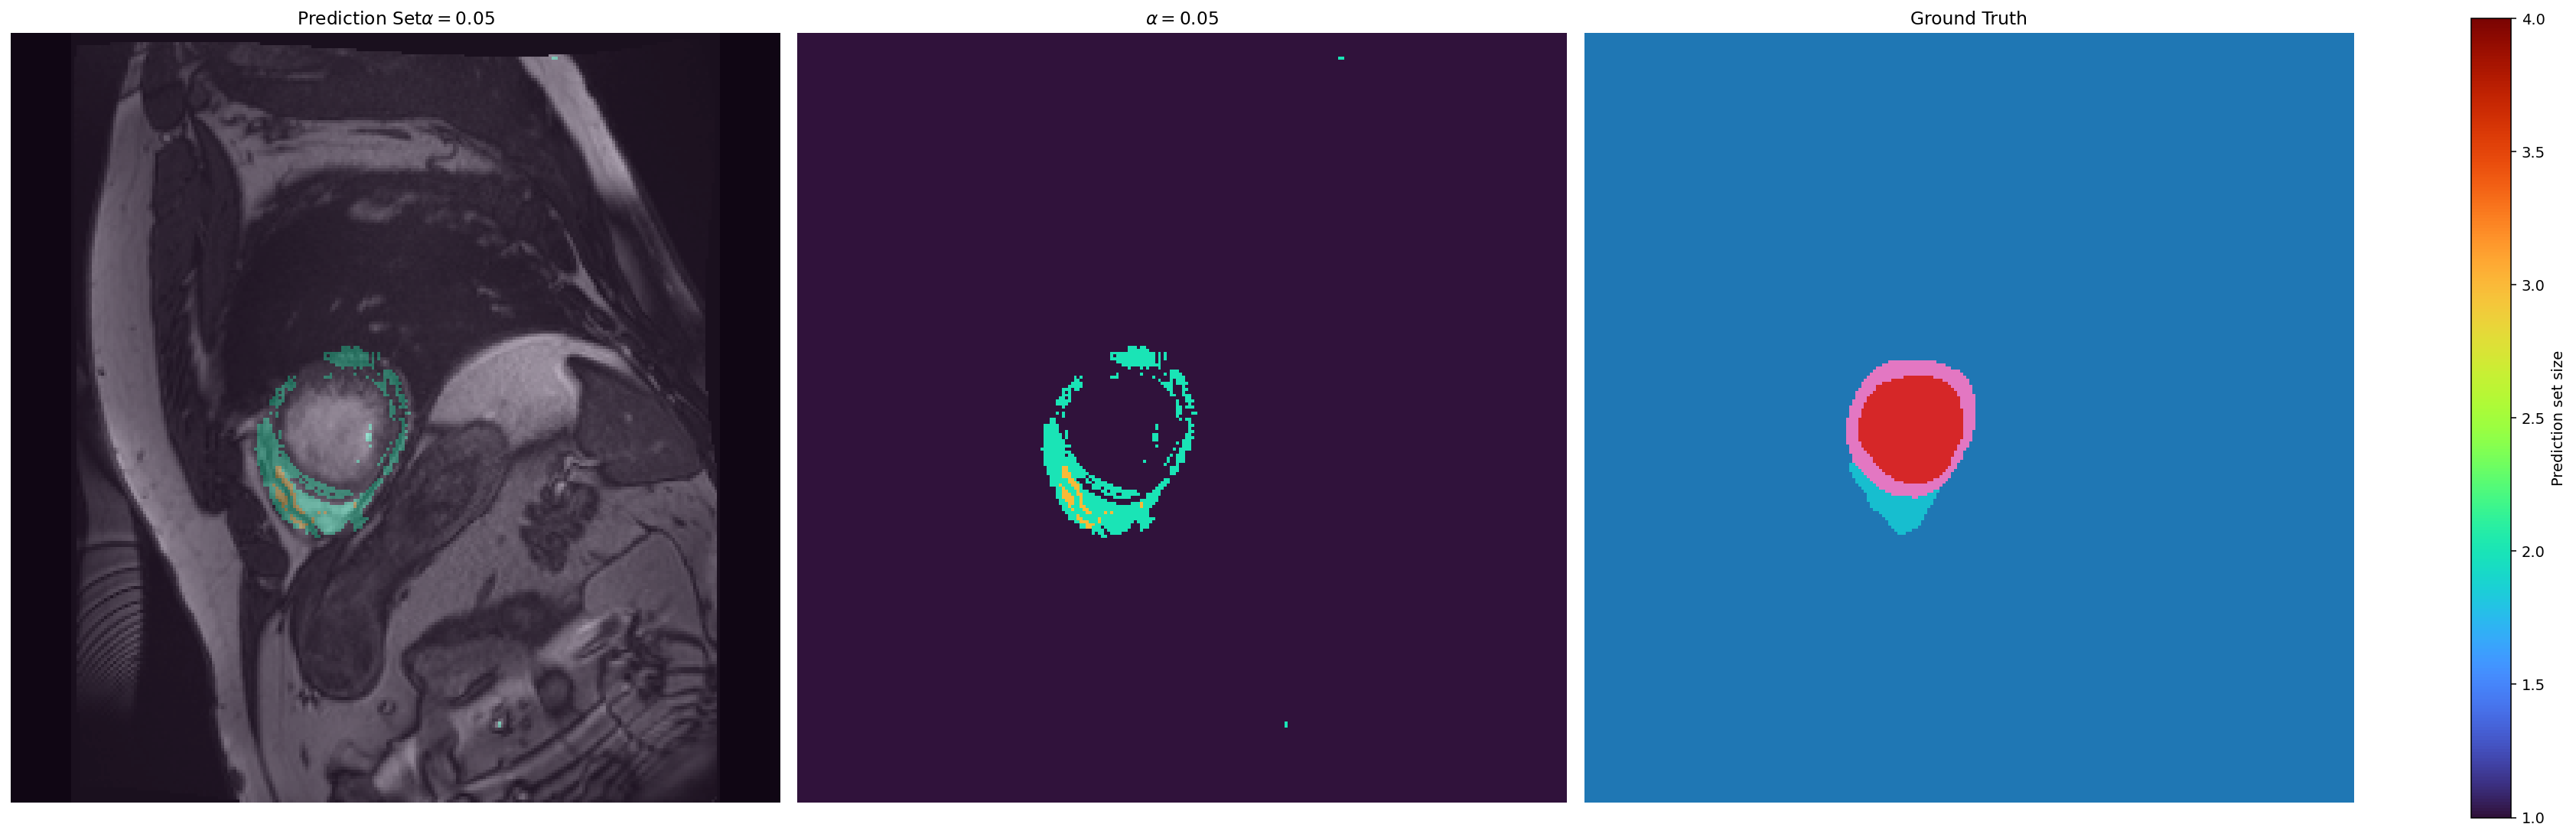
\includegraphics[width=1\linewidth]{img/prediccion_desv.png}
    \caption{Predicción, incerteza y grouth true}
    \label{fig:pred_desv}
\end{figure}

\begin{figure}[H]
    \centering
    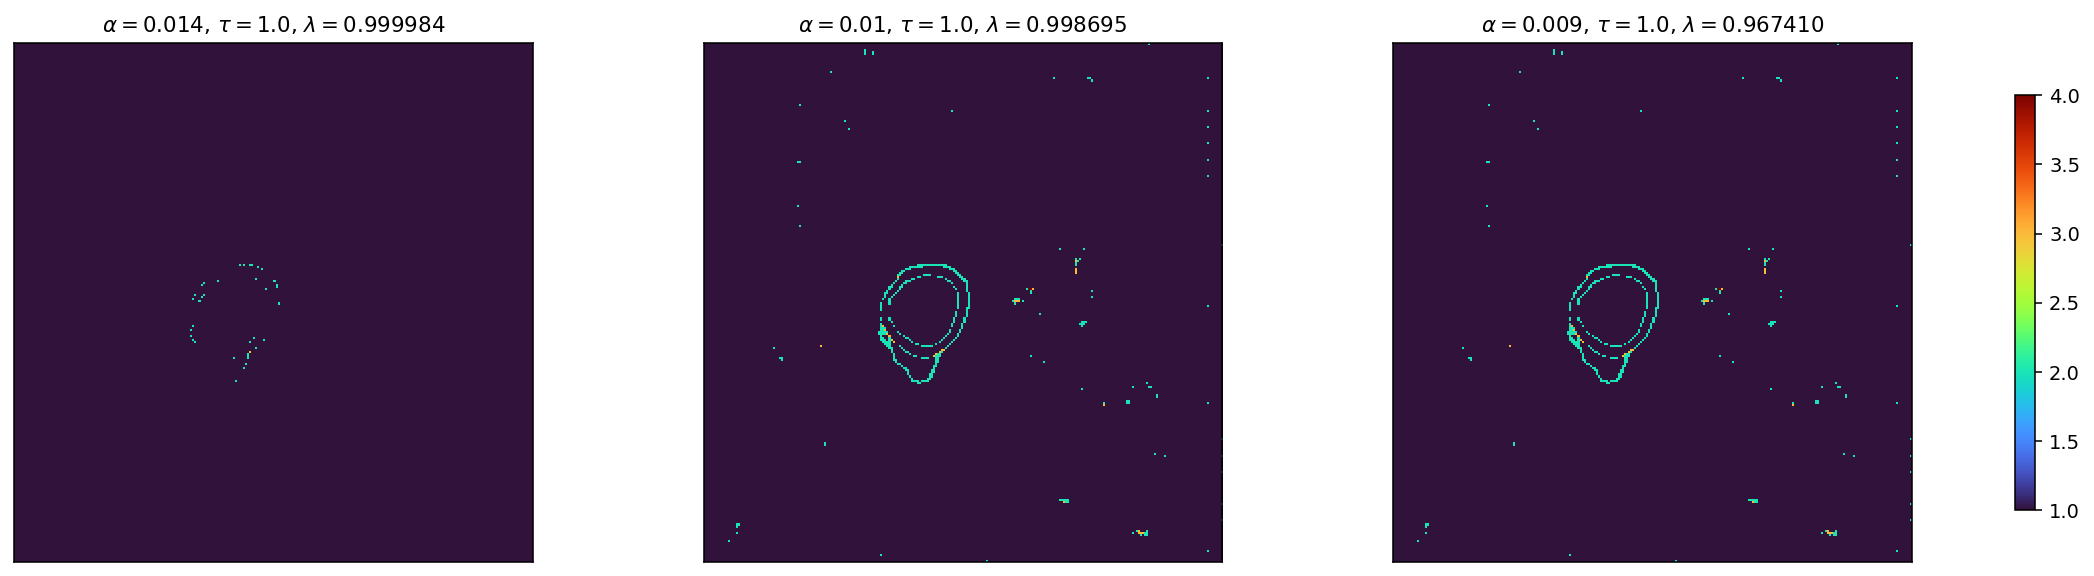
\includegraphics[width=1\linewidth]{img/variando_alphas.png}
    \caption{Incertidumbre del modelo para alphas [0.014, 0.01, 0.0090] y la temperatura $\tau = 1.0$ }
    \label{fig:desviacion_alphas}
\end{figure}

Las regiones de predicción se construyen agregando, píxel a píxel, todas las clases cuyas probabilidades predichas superen el umbral $1 - \hat{\lambda}$. Adicionalmente, se incluye de forma determinista la clase con la mayor probabilidad estimada en cada caso; esta modificación técnica previene la obtención de conjuntos vacíos en regímenes donde el umbral de aceptación resulta excesivamente estricto (valores de $\hat{\lambda}$ muy pequeños).

\section{Cuantificación de incertidumbre para imágenes médicas mediante FBPINN}

En esta sección se aborda la cuantificación de la incertidumbre en un conjunto de datos de imágenes de estructuras vasculares (venas). Estas imágenes fueron reconstruidas a través de un modelo de Redes Neuronales Informadas por la Física (PINN); en particular, se empleó la arquitectura de PINN Basada en Bases Finitas (FBPINN).

Como se describió previamente, la aplicación de la predicción conforme requiere definir inicialmente una función de puntuación de no conformidad. Para este propósito, se propone utilizar la norma $\mathbb{L}_1$, definida formalmente como:
\begin{equation}
    S = |y - \hat{y}|
\end{equation}

\begin{figure}[H]
    \centering
    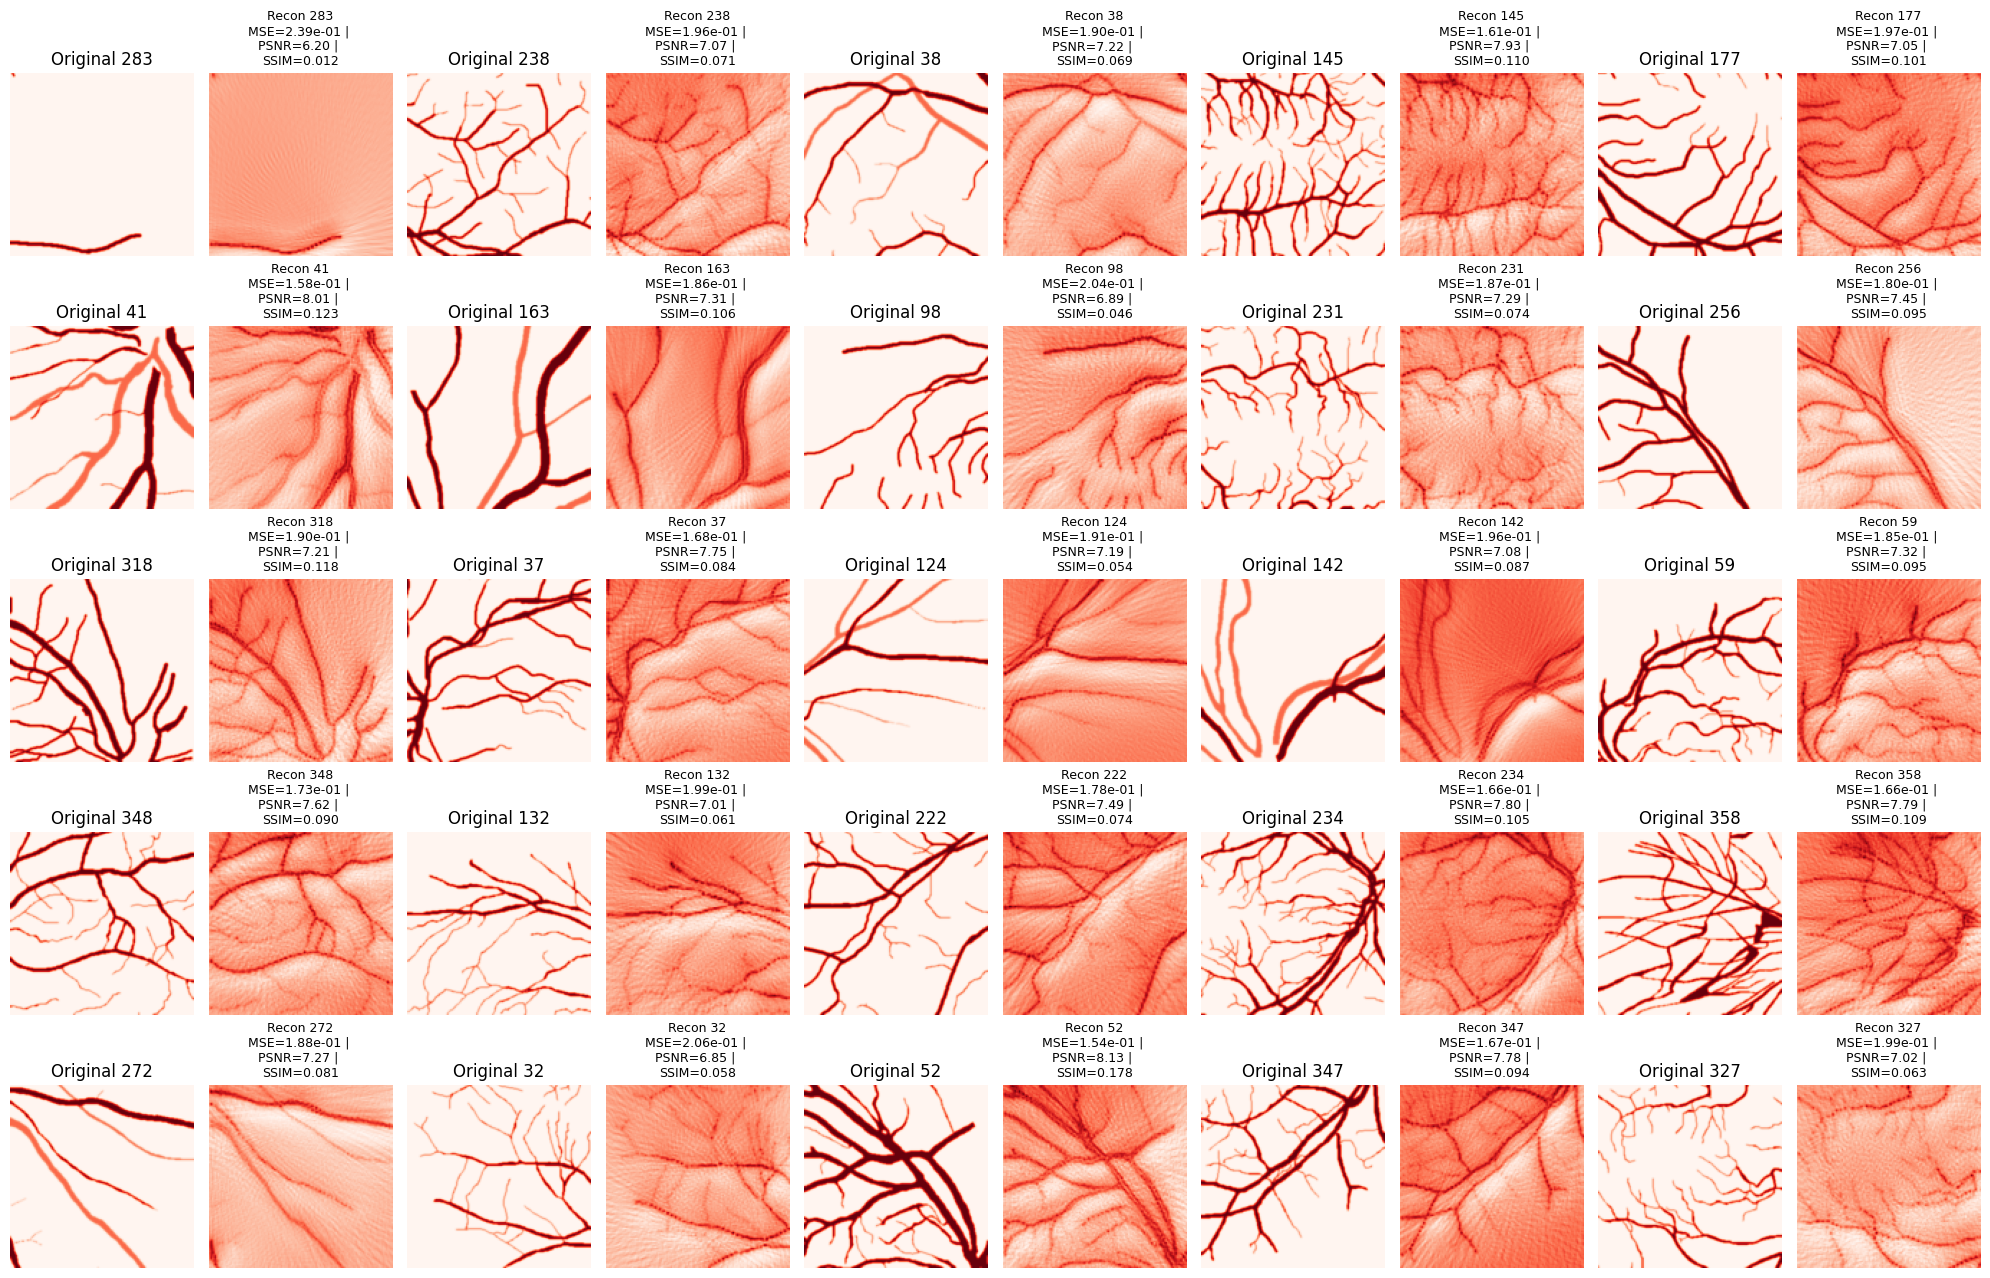
\includegraphics[width=1\linewidth]{img/data_init.png}
    \caption{Imágenes médicas reconstruidas mediante FBPINN y resolución del problema inverso.}
    \label{fig:data_fbpinn}
\end{figure}

Es fundamental destacar que el modelo no toma como entrada la imagen original directamente, sino una reconstrucción fundamentada en funciones gaussianas. El operador aprende a reconstruir la onda acústica a través del pulso gaussiano aplicándolo a cada coordenada espacial de la imagen, generando así un sinograma. Posteriormente, este sinograma es procesado por un algoritmo determinista que resuelve el problema inverso para reconstruir la imagen final.

Por lo tanto, la entrada efectiva al modelo se denota como $y_{\text{reconstruida}} = p_0$, la cual representa una matriz espacial con los valores de presión inicial para cada píxel. Sobre esta base, se procede a aplicar un conjunto de algoritmos de predicción conforme con carácter exploratorio.

\subsection{Split Conformal Prediction (SCP) en FBPINN}

En primera instancia, se evalúa el algoritmo SCP aplicado de forma independiente píxel a píxel, modalidad que se denota en la literatura como calibración condicional local. Es imperativo resaltar que el algoritmo SCP convencional ofrece, por definición, una garantía de cobertura marginal; es decir, el nivel de confianza se cumple en el promedio de la imagen y no necesariamente de manera condicional para cada píxel de forma aislada.

Para mitigar la varianza en la estimación de los cuantiles locales y aproximar una cobertura condicional robusta, se requiere disponer de un volumen considerable de muestras en el conjunto de calibración.

\begin{figure}[H]
    \centering
    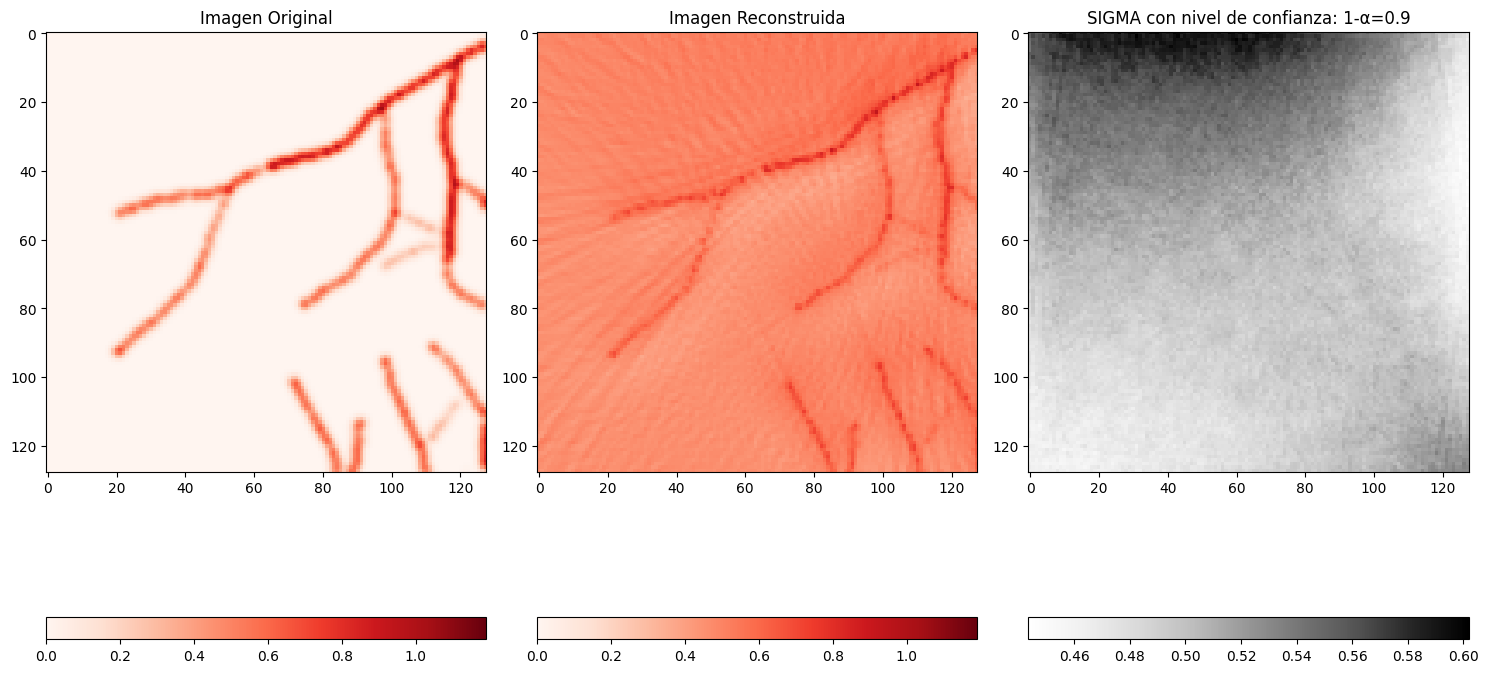
\includegraphics[width=0.8\linewidth]{img/scp_fbpinn.png}
    \caption{Split Conformal Prediction aplicado bajo calibración condicional, donde $\sigma = \hat{q}$.}
    \label{fig:scp_fbpinn}
\end{figure}

Un aspecto analítico relevante observado en la Figura~\ref{fig:scp_fbpinn} es que el umbral $\hat{q}$ deja de ser un escalar constante para todo el dominio. En su lugar, se transforma en una matriz que preserva la dimensión espacial de la imagen, de modo que $\hat{q} \in \mathbb{R}^{H \times W}$.

Esta técnica proporciona una caracterización topográfica general de la incertidumbre a lo largo de la malla de píxeles, permitiendo formular una región de predicción conforme de la forma $\hat{f}(X_{\text{test}}) \pm \hat{q}$. No obstante, estos intervalos de confianza resultan idénticos para cualquier instancia del conjunto de prueba $(\mathcal{X}, \mathcal{Y})_{\frac{n}{2} + 1, \dots, n}$, a pesar de que la física del problema sugiere que la incertidumbre debería exhibir variaciones dinámicas entre imágenes.

Con el objetivo de introducir dependencia de la muestra en la inferencia, e inspirándonos en el método de puntuación por residuo escalado, se propone una modificación adaptativa. Mientras que la etapa de calibración permanece invariante, la incertidumbre resultante para la fase de prueba se escala mediante la siguiente formulación:

\begin{equation}
    \sigma_q = \frac{q(i,j)^{\alpha}}{\mathcal{\hat{\pi}}(y \in \mathcal{R}_1|x)(i,j)}
\end{equation}

Donde el término $\mathcal{\hat{\pi}}(y \in \mathcal{R}_1|x)(i,j)$ representa la probabilidad condicional de que el píxel en la coordenada $(i,j)$ pertenezca a la estructura vascular (vena), $q(i,j)^{\alpha}$ es debido a que por cada $\alpha$ seteado se obtendrá una nueva matriz de $q(i,j)$.

Para estimar esta distribución, la imagen se segmenta mediante el algoritmo de Expectación-Maximización (EM) usando mezcla de gaussiandas  sobre el espacio de intensidades de los píxeles los cuales fueron clusterizados con y sin ecualización previa.

El proceso consiste en normalizar las intensidades del histograma al intervalo $[0, 255]$ para posteriormente ajustar el modelo de mixturas que infiere la probabilidad píxel a píxel. Esta probabilidad actúa como una máscara adaptativa que genera regiones de incertidumbre dinámicas y específicas para cada imagen de prueba.

\begin{figure}[H]
    \centering
    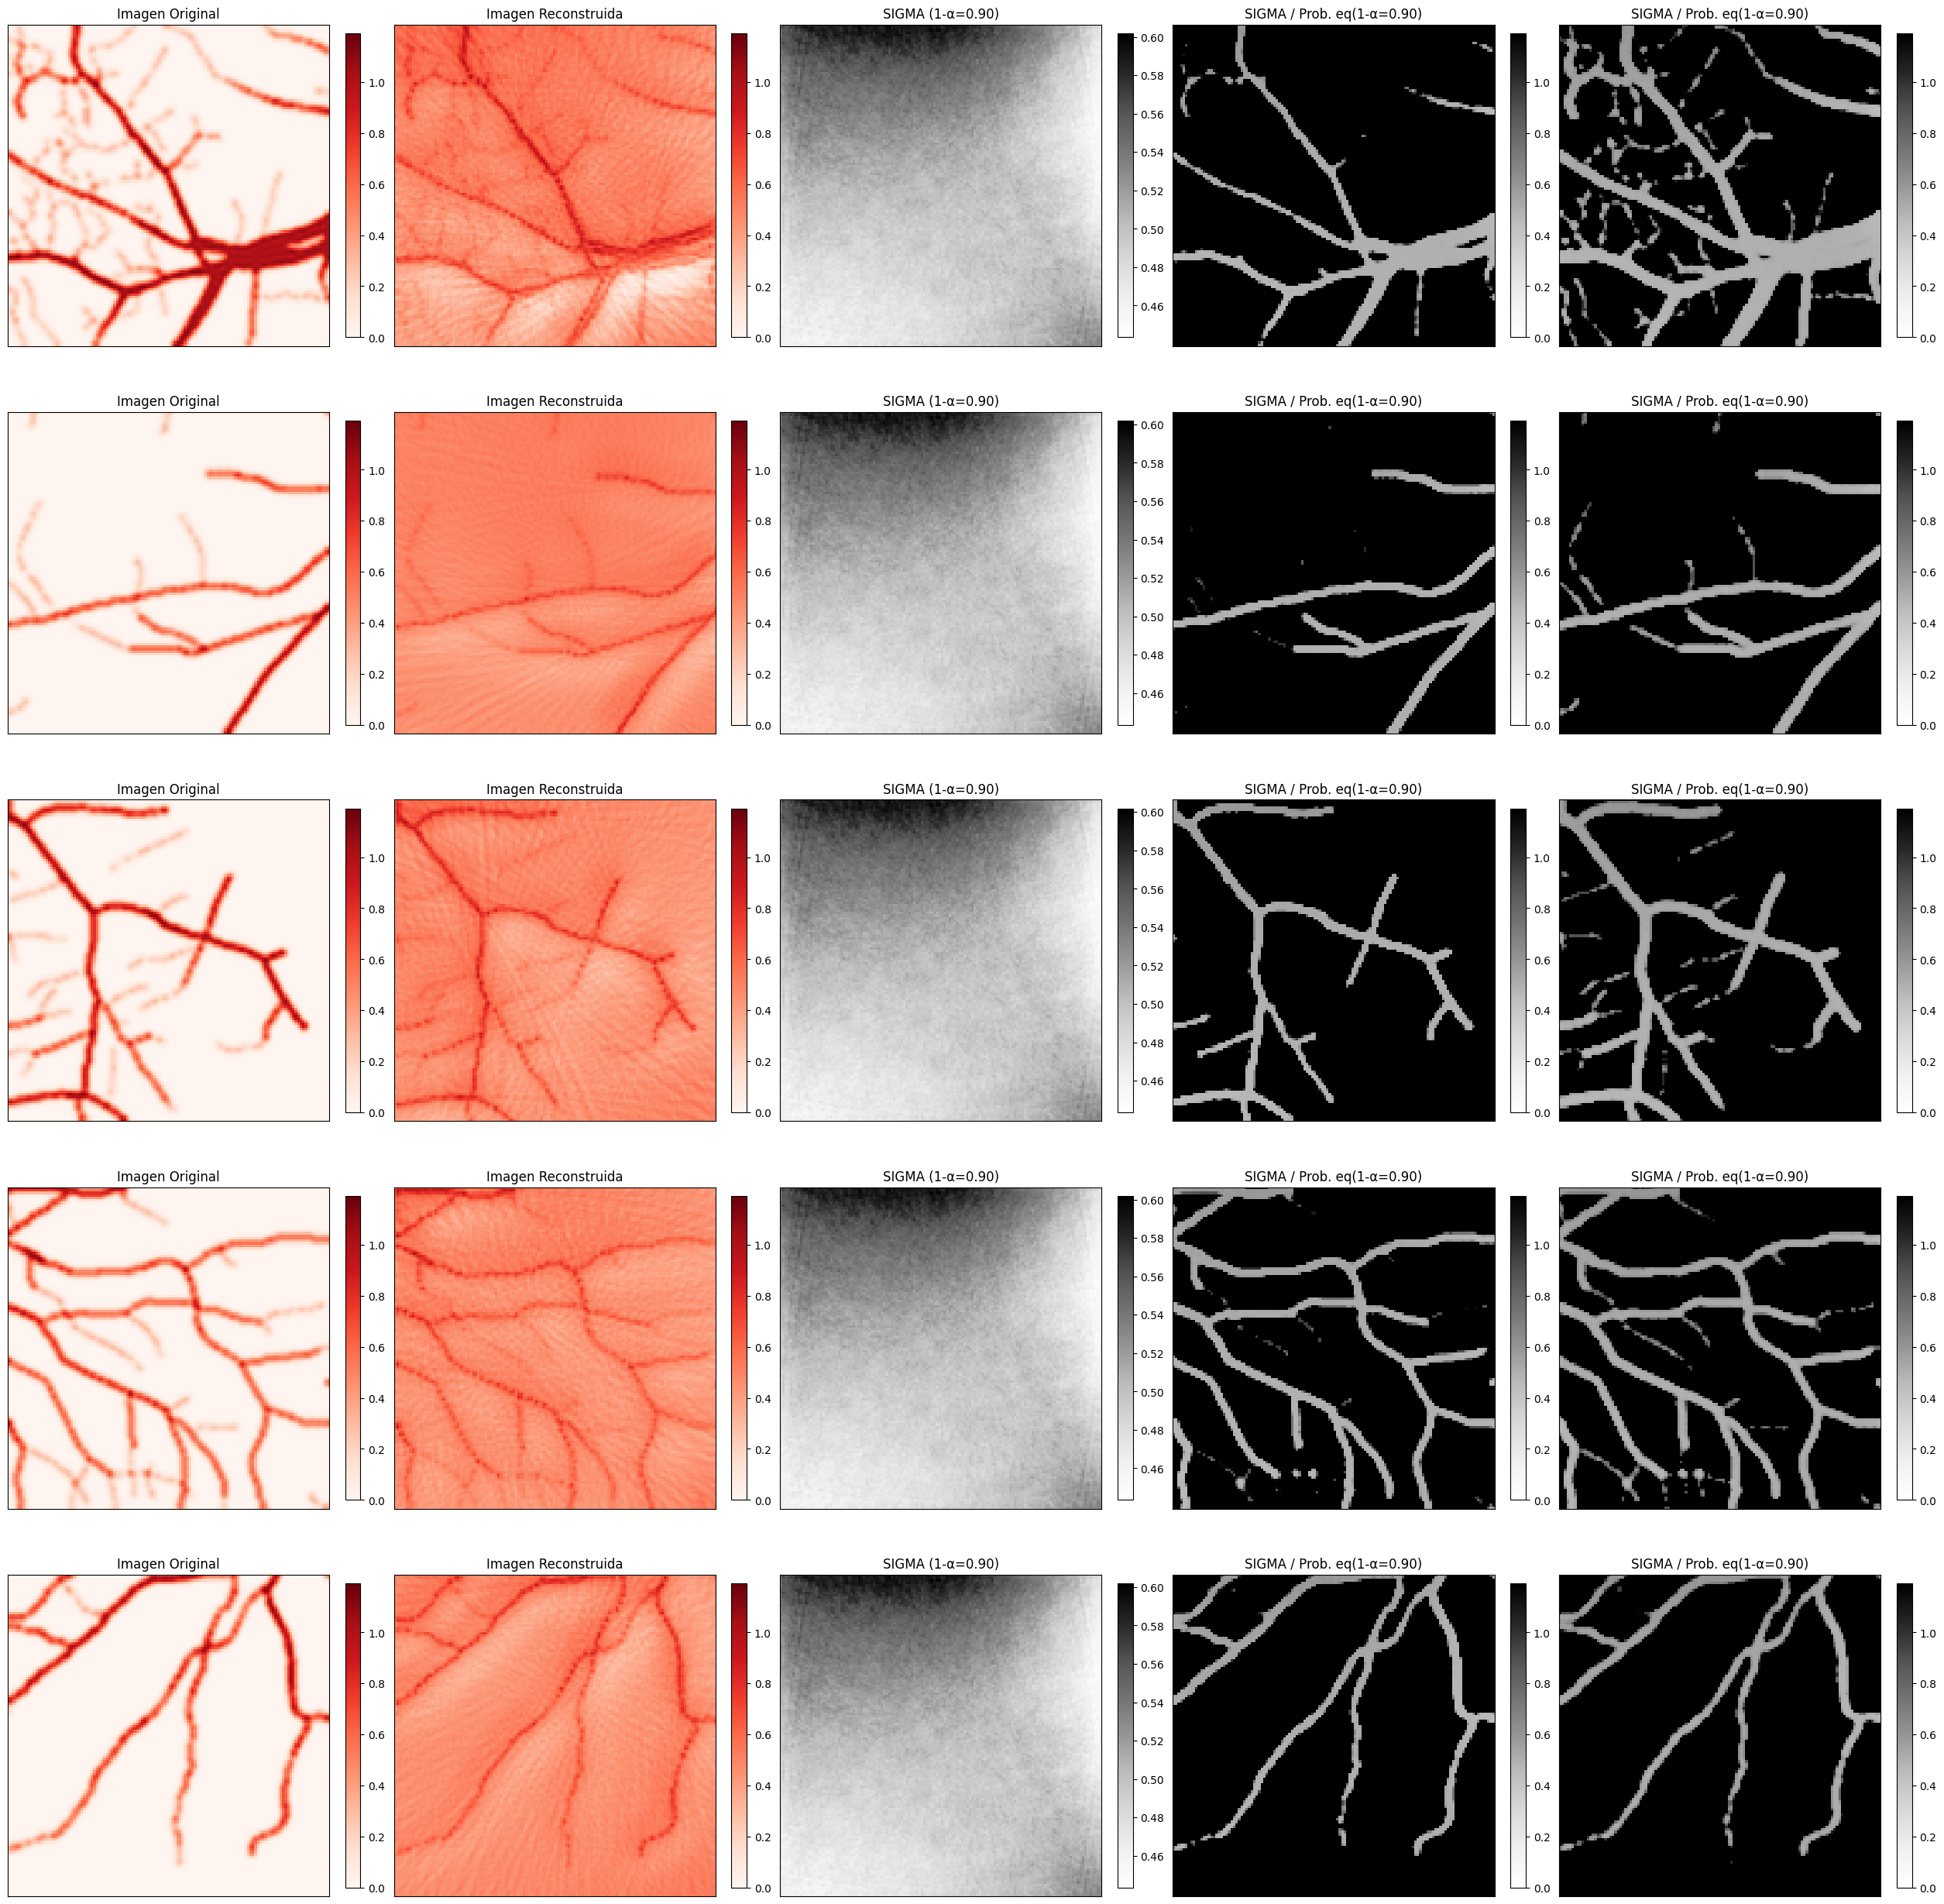
\includegraphics[width=0.75\linewidth]{img/scp_conf_EM.png}
    \caption{Split Conformal Prediction con bandas de predicción escaladas mediante la máscara de probabilidad EM.}
    \label{fig:scp_mascara}
\end{figure}

\subsection{SCP basado en partición binaria de clases}

A partir de la capacidad de segmentación introducida en el enfoque anterior, surge la oportunidad estratégica de fragmentar el dominio de calibración. Específicamente, se propone aplicar SCP condicional de forma aislada para el conjunto de píxeles clasificados como estructuras vasculares, y un proceso homólogo e independiente para los píxeles asignados al fondo.

Bajo este esquema, el dominio espacial se particiona en dos subconjuntos disjuntos a los cuales se les induce un proceso de calibración conforme por separado.

\begin{figure}[H]
    \centering
    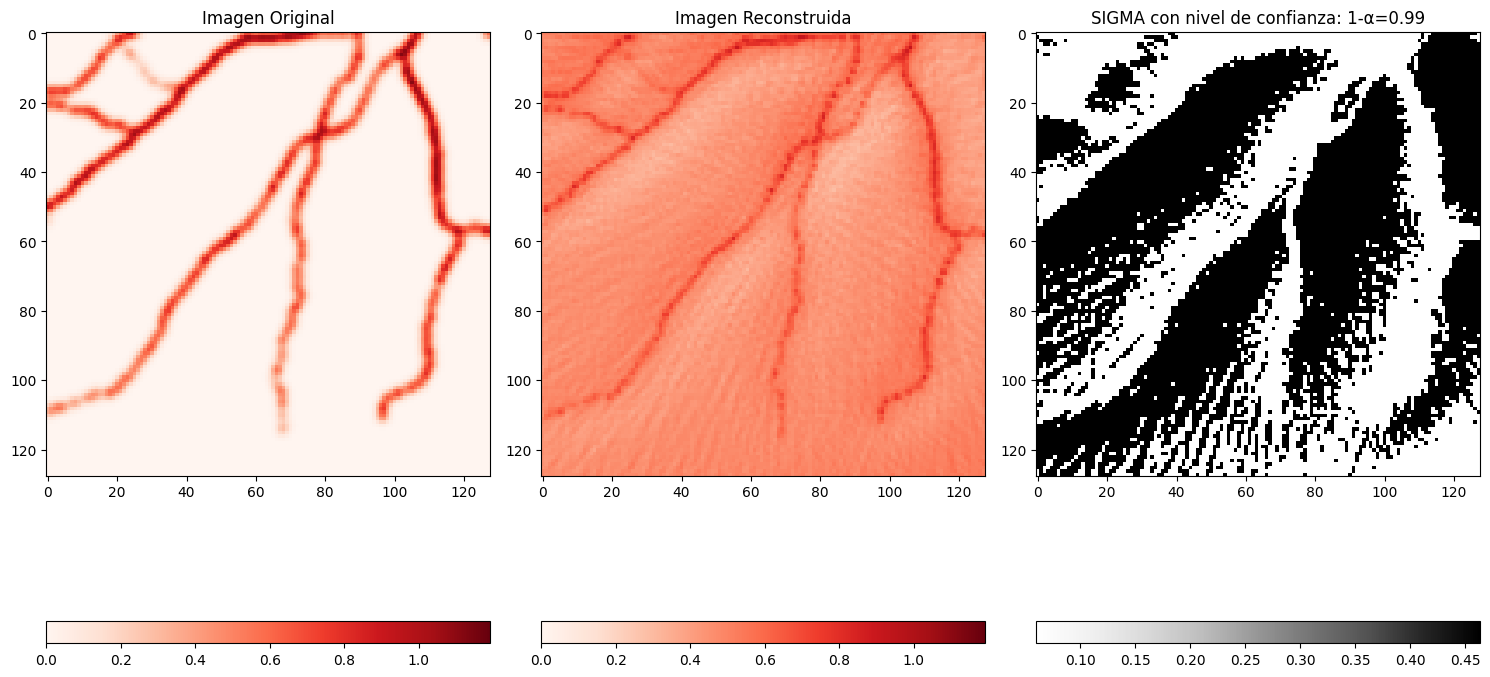
\includegraphics[width=0.75\linewidth]{img/scp_doble_em.png}
    \caption{Esquema de doble Split Conformal Prediction aplicado de forma independiente a las regiones de vena y fondo.}
    \label{fig:doble_scp_cluster}
\end{figure}

Este enfoque binario permite restringir el tamaño de los intervalos, logrando disminuir significativamente la incertidumbre en las regiones donde no se compromete la presencia de estructuras vasculares.

\subsection{Método de Kandinsky}

El método de Kandinsky, concebido originalmente para escenarios de clasificación, busca armonizar las ventajas de la calibración condicional local y la calibración marginal, tal como se detalla en el algoritmo~\ref{alg:kandinsky}. A través de un enfoque basado en agrupamiento espacial y pooling de puntuaciones de no conformidad, el método viabiliza estimaciones estables y estadísticamente válidas en dimensiones espaciales de alta resolución.

\begin{algorithm}[H]
    \caption{Algoritmo de Kandinsky Conformal Prediction}
    \label{alg:kandinsky}
    \begin{algorithmic}[1]
        \REQUIRE Tensor de no conformidad de calibración $\mathbf{S} \in \mathbb{R}^{N \times H \times W}$, niveles de cuantiles discretos $\mathcal{Q} = \{\tau_1, \dots, \tau_M\}$, número de clústeres $K$, nivel de significancia $\alpha$, instancia de prueba $X_{\text{test}}$.
        \ENSURE Mapa topográfico de umbrales $\mathbf{Q} \in \mathbb{R}^{H \times W}$, conjuntos de predicción válidos $\mathcal{C}_{\alpha}(X_{\text{test}})$.

        \vspace{0.1cm}
        \STATE \textbf{// Fase I: Extracción de Características Locales}
        \FOR{cada coordenada espacial $(i, j) \in \{1, \dots, H\} \times \{1, \dots, W\}$}
            \STATE Inicializar vector de perfil de riesgo: $\mathbf{x}_{i,j} \in \mathbb{R}^M$
            \FOR{$m = 1$ \TO $M$}
                \STATE $\mathbf{x}_{i,j}[m] \leftarrow \inf \left\{ q \in \mathbb{R} : \frac{1}{N} \sum_{n=1}^N \mathbb{I}(S_{n,i,j} \leq q) \geq \tau_m \right\}$
            \ENDFOR
        \ENDFOR
        \STATE Construir la matriz global de diseño: $\mathbf{X} \leftarrow \big[\mathbf{x}_{1,1}, \dots, \mathbf{x}_{H,W}\big]^T \in \mathbb{R}^{(H \cdot W) \times M}$

        \vspace{0.1cm}
        \STATE \textbf{// Fase II: Agrupamiento Espacial (Clustering)}
        \STATE Calcular la partición del dominio $\pi: \{1, \dots, H\} \times \{1, \dots, W\} \to \{1, \dots, K\}$ vía Clustering($\mathbf{X}, K$)
        \STATE Asignar la máscara estática de Kandinsky $\mathbf{M} \in \{1, \dots, K\}^{H \times W}$ tal que $\mathbf{M}_{i,j} \leftarrow \pi(i,j)$

        \vspace{0.1cm}
        \STATE \textbf{// Fase III: Calibración Regional (Pooling)}
        \FOR{cada índice de clúster $k = 1$ \TO $K$}
            \STATE Agregar el multiconjunto de puntuaciones históricas: $\mathcal{S}_k \leftarrow \Big\{ S_{n,i,j} \;\Big|\; n \in \{1, \dots, N\}, \; \mathbf{M}_{i,j} = k \Big\}$
            \STATE Determinar el tamaño muestral efectivo regional: $N_k \leftarrow |\mathcal{S}_k| $
            \STATE Calcular el cuantil corregido: $q_k^* \leftarrow \inf \left\{ q \in \mathbb{R} : \frac{1}{N_k} \sum_{s \in \mathcal{S}_k} \mathbb{I}(s \leq q) \geq \frac{\lceil (N_k + 1)(1 - \alpha) \rceil}{N_k} \right\}$
        \ENDFOR

        \vspace{0.1cm}
        \STATE \textbf{// Fase IV: Inferencia Estática y Proyección}
        \STATE Proyectar mapa de umbrales: $\mathbf{Q}_{i,j} \leftarrow \sum_{k=1}^K q_k^* \cdot \mathbb{I}(\mathbf{M}_{i,j} = k) \quad \forall (i,j)$
        \FOR{cada píxel $(i, j) \in X_{\text{test}}$}
            \STATE $\mathcal{C}_{\alpha}(X_{\text{test}})_{i,j} \leftarrow \left\{ y \in \{1, \dots, \mathcal{Y}\} : 1 - \hat{f}(X_{\text{test}})_{i,j,y} \leq \mathbf{Q}_{i,j} \right\}$
        \ENDFOR

        \RETURN $\mathbf{Q}$, $\mathcal{C}_{\alpha}(X_{\text{test}})$
    \end{algorithmic}
\end{algorithm}

Si bien el algoritmo de Kandinsky fue concebido originalmente para problemas de clasificación, su formulación matemática permite extenderlo de manera directa al ámbito de la regresión. Dado que el método opera fundamentalmente sobre la distribución espacial de las puntuaciones de no conformidad, las funciones de score continuas provenientes de un regresor base pueden ser integradas y calibradas bajo los mismos principios de agregación regional y agrupamiento espacial descritos en las secciones anteriores.

\begin{figure}[H]
    \centering
    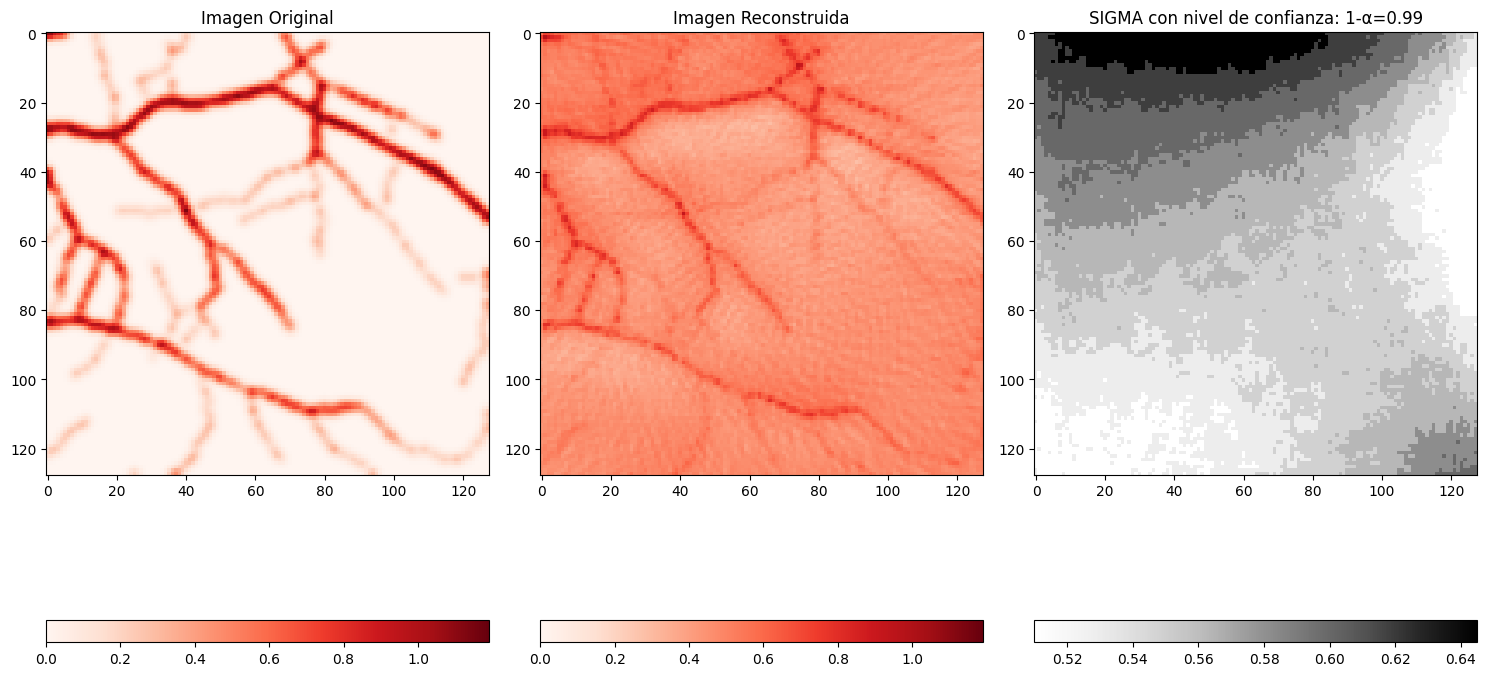
\includegraphics[width=0.75\linewidth]{img/kandinsky.png}
    \caption{Kandinsky conformal predictión}
    \label{fig:kandinsky}
\end{figure}


En la primera fase, el método condensa la información del conjunto de calibración calculando $M$ cuantiles empíricos de forma local para cada píxel. De este modo, se transforma el histórico dimensional de errores en una matriz espacial de características exógenas donde cada coordenada geométrica queda representada por un vector que describe su perfil de riesgo local.

Posteriormente, en la segunda fase, estos vectores de cuantiles actúan como las características de entrada para un algoritmo de agrupamiento parametrizado con $K$ clases, lo que permite segmentar y particionar el dominio de la imagen en una máscara estática que unifica los píxeles con dinámicas de incertidumbre estadísticamente similares.

En la tercera fase, se ejecuta un proceso de recalibración independiente sobre los componentes de cada clúster; al agregar las puntuaciones de no conformidad de todos los píxeles pertenecientes a una misma región a lo largo de todas las muestras de calibración, se produce un aumento masivo de datos que estabiliza el tamaño muestral efectivo. Este mecanismo de agregación regional no solo optimiza la precisión en la estimación del cuantil conforme global, sino que además mitiga de manera drástica el ruido heterocedástico local de alta frecuencia.

Finalmente, durante la etapa de inferencia, la predicción de cualquier instancia futura se realiza proyectando los scores del modelo sobre el mapa de umbrales estáticos e invariantes derivado de los datos aumentados, garantizando así la estabilidad y robustez de la cobertura condicional por zona.




 %3. Propiedades Matemáticas
%*   **Simetría:** En el procedimiento de "Full Conformal", se requiere que la función de puntuación sea **simétrica**, lo que significa que su valor debe ser invariante ante permutaciones del orden de los datos en el conjunto de entrenamiento $D$.
%*   **Relación con los cuantiles:** La fase de inferencia consiste en recolectar todos los valores de $y$ cuyo score $s(X_{test}, y)$ sea menor o igual a un **cuantil crítico ($\hat{q}$)** calculado previamente sobre un conjunto de calibración.

%*   **Interpretación como p-valor:** Los scores permiten definir un **p-valor conforme** ($p^y$), que mide la fracción de scores de entrenamiento que son mayores o iguales al score del punto de prueba hipotético. Si este p-valor es mayor que el nivel de error $\alpha$, el valor se incluye en el conjunto de predicción.









%revisar la expresion de cuantiles
